\section{Protein relocalisation}


\begin{frame}{Spatial dynamics}
  \begin{block}{Trans-localisation event during monocyte to macrophage
      differentiation}
    Investigate the effect of lipopolysaccharides (LPS)-mediated
    inflammatory response in human monocytic cells (THP-1)
  \end{block}

  \begin{block}{Data}
    \begin{itemize}
    \item Triplicate \textbf{temporal} profiling (0, 2, 4, 6, 12, 24
      hours).
    \item Triplicate \textbf{spatial} profiling (0 vs 12 hours) -
      early trafficking, before actual morphological differentiation
      at 24h.
    \end{itemize}
  \end{block}

  Work lead by \textbf{Dr Claire Mulvey} at the Cambridge Centre for
  Proteomics.

\end{frame}



\begin{frame}
  \begin{figure}[h]
    \centering
    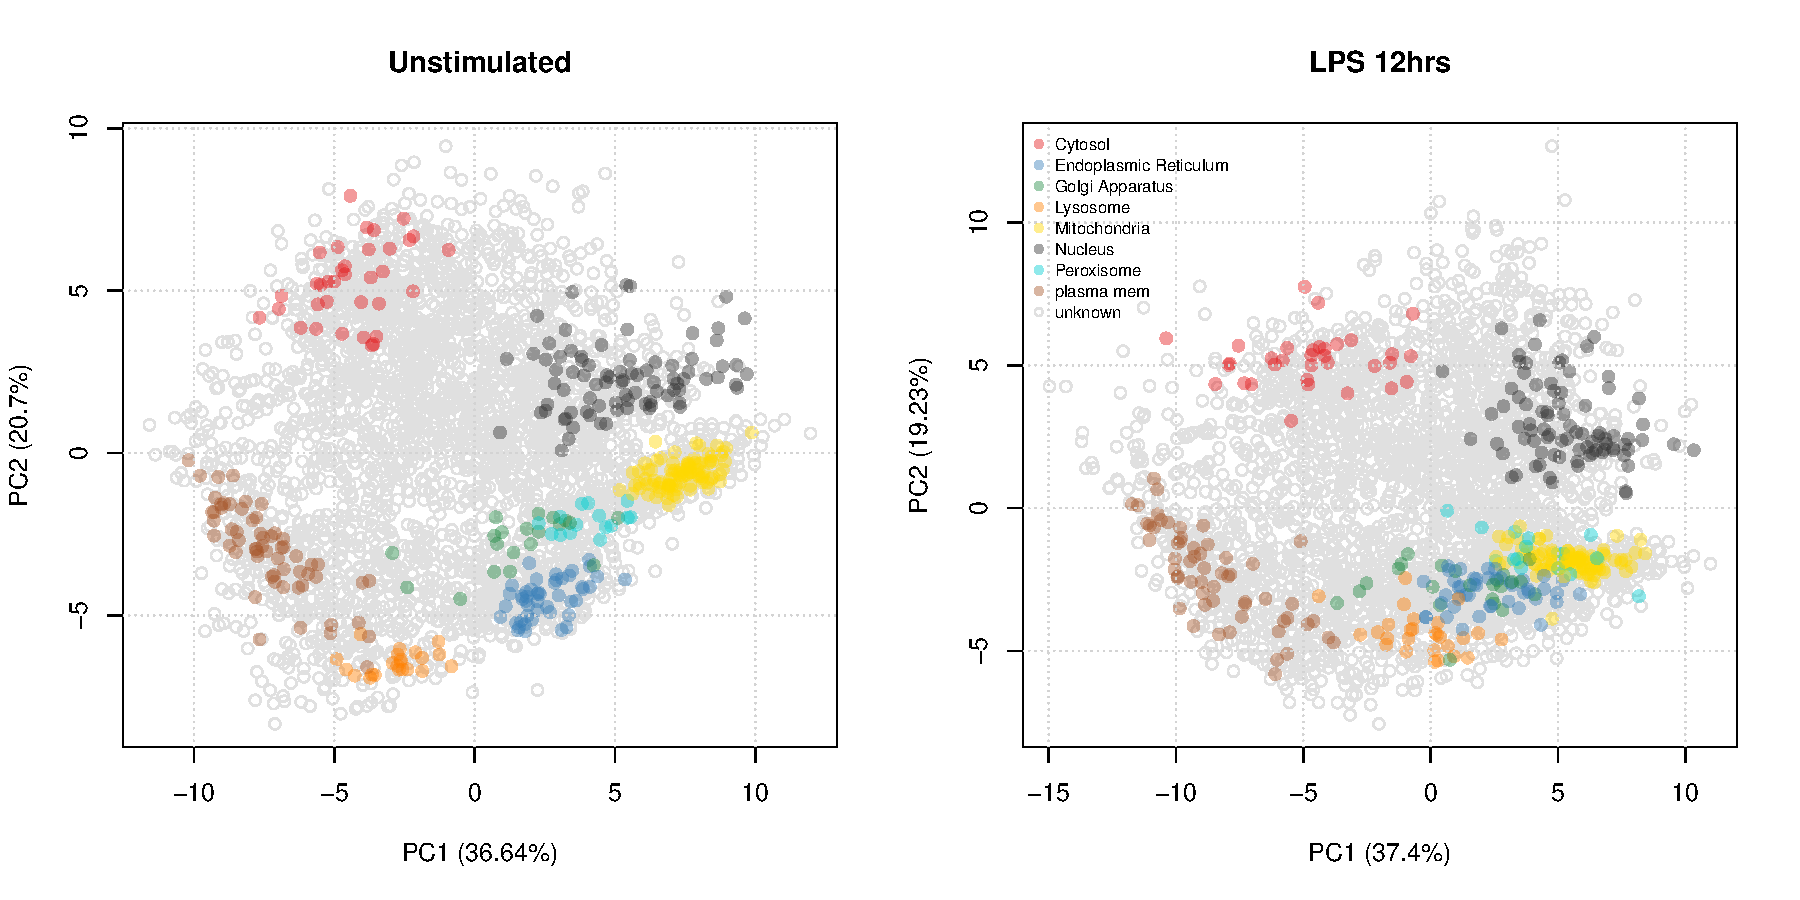
\includegraphics[width=\linewidth]{./figs/lps.pdf}
    \caption{Spatial maps of unstimulated and LPS-treated cells
      (combined triplicates).}
  \end{figure}
\end{frame}

\begin{frame}
  \begin{figure}[h]
    \centering
    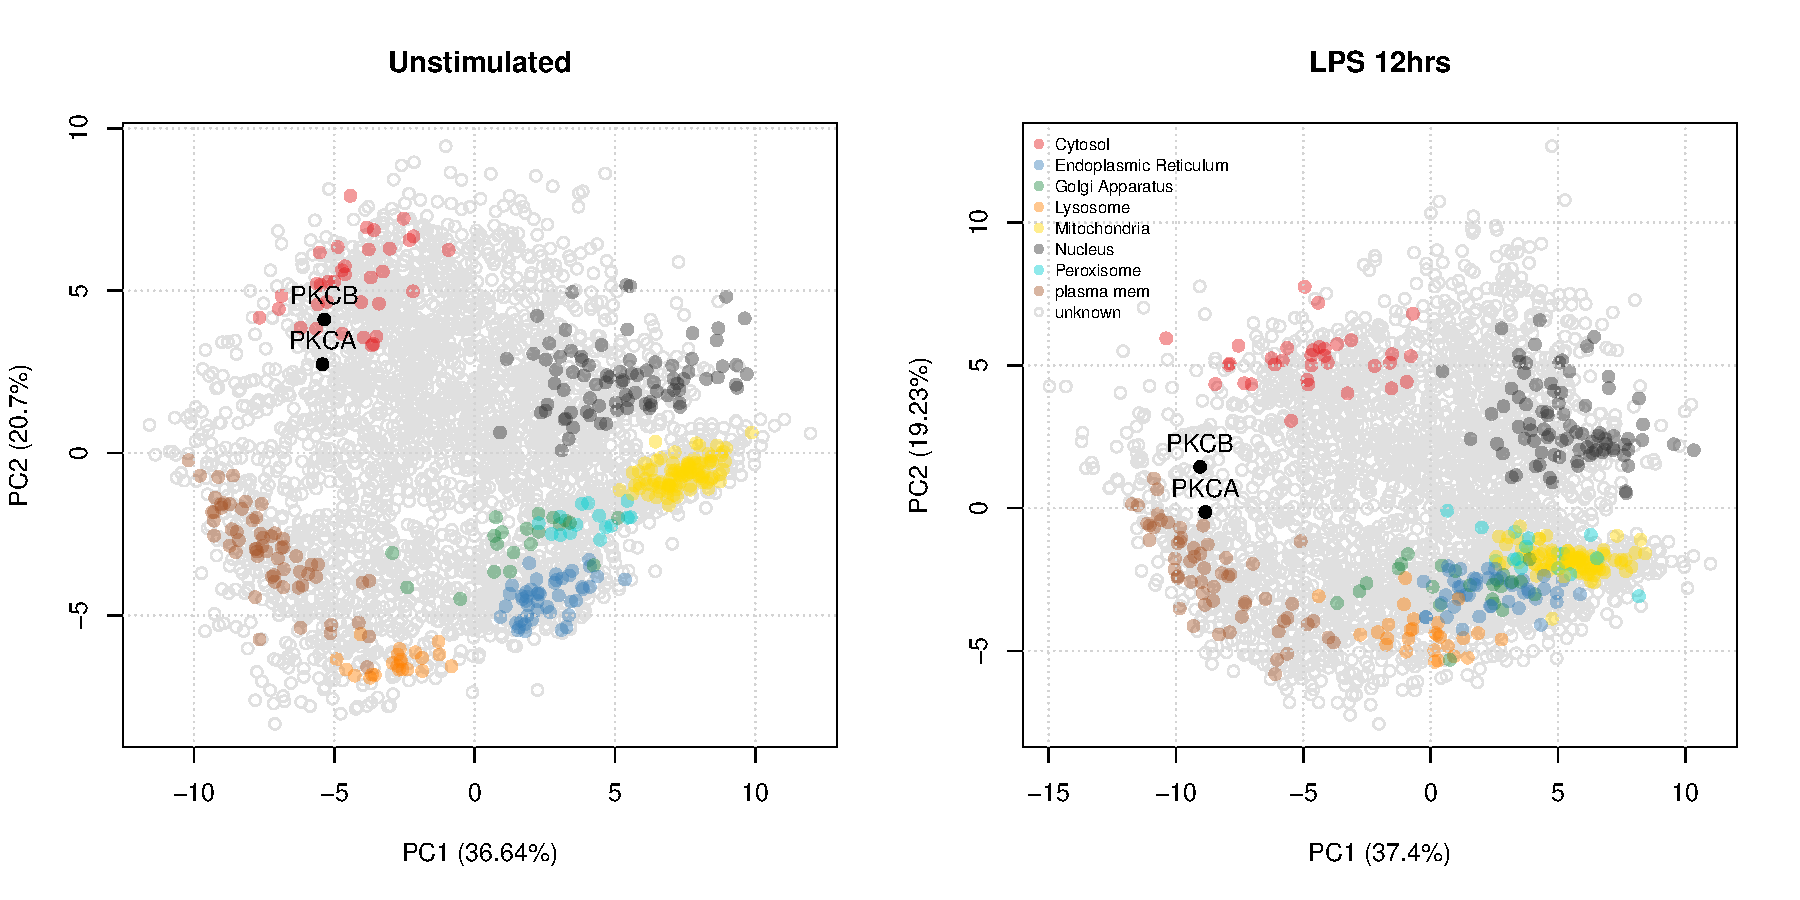
\includegraphics[width=\linewidth]{./figs/lps-pkc.pdf}
    \caption{Relocation of Protein Kinase C $\alpha$ and $\beta$ from the
      cytosol to the plasma membrane, \textbf{driving maturation into
        a differentiated macrophage phenotype}.}
  \end{figure}
\end{frame}

\begin{frame}
  \begin{figure}[h]
    \centering
    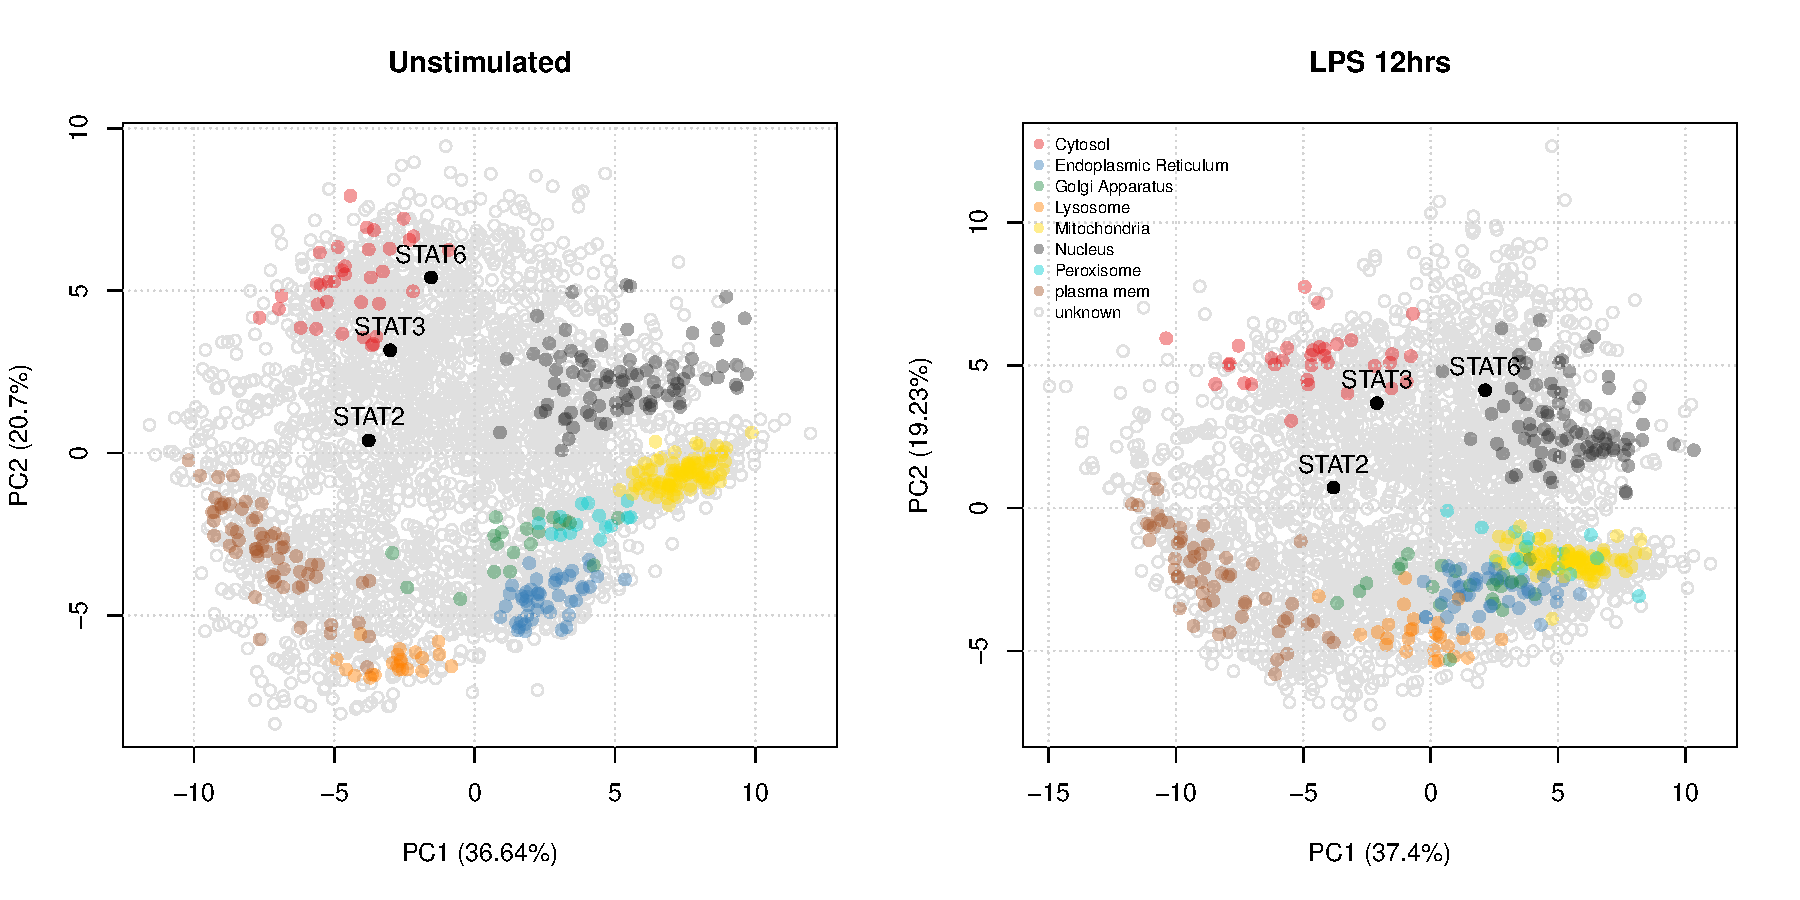
\includegraphics[width=\linewidth]{./figs/lps-stat.pdf}
    \caption{Relocation of Signal transducer and activator of
      transcription 6 (STAT6) from the cytosol to the Nucleus,
      \textbf{activating anti-bacterial and anti-viral-like
        response}. Validated by microscopy and see also
      \cite{Chen:2011}.}
  \end{figure}
\end{frame}



\begin{frame}
  \begin{block}{Folding and stability}
      \begin{itemize}
      \item Re-localisation upon protein post-translational modification (PTM).
      \item Effect of PTM on protein 3D structure.
      \item Link between 3D structure and localisation.
      \end{itemize}
  \end{block}
\end{frame}
